\documentclass[a4pper,11pt]{article}
\usepackage{lipsum} %This package just generates Lorem Ipsum filler text. 
\usepackage{graphicx}
\usepackage{natbib}
\usepackage{geometry}
\usepackage[english]{babel}
\usepackage[utf8]{inputenc}
\usepackage[linesnumbered,ruled,vlined]{algorithm2e}
\usepackage[noend]{algpseudocode}
\usepackage[usenames]{color}
\usepackage{amsmath,amsthm,amssymb,amsfonts}
\usepackage{dsfont}
\usepackage{mathrsfs}
\usepackage{tabu}
\usepackage{multirow}
\usepackage{enumerate}
\usepackage{listings}
\usepackage{subfigure}
\usepackage{float}
\usepackage{authblk}
\usepackage{bm}
\usepackage{calligra}
% my cmd
%%%%%%%%%%%%%%%%
% start my commands
%%%%%%%%%%%%%%%%
\newcommand{\lm}{\lambda_\textrm{max}}
\newcommand{\trace}{\mathbf{trace}}
\newcommand{\diag}{\mathbf{diag}}
\newcommand{\model}[1]{(\textbf{#1})}
\newcommand{\mx}{\mathbf{\max}\;}
\newcommand{\mn}{\mathbf{\min}\;}
\newcommand{\st}{\mathrm{s.t.\;}}
\newcommand{\ex}{\mathbb E}
\newcommand{\dx}{\;\bm dx}
\newcommand{\pr}{\mathbb P}
\newcommand{\id}{\mathbb I}
\newcommand{\bp}{\mathbb P}
\newcommand{\be}{\mathbb E}
\newcommand{\bi}{\mathbb I}
\newcommand{\bxi}{\bm \xi}
\newcommand{\bo}{\bm \omega}
\newcommand{\va}{\mathbf{Var}}
\newcommand{\dif}{\mathbf{d}}
\newcommand{\minp}[2]{\min\{#1, #2\}}
\newcommand{\intp}{\mathbf{int}}
\newcommand{\apex}{\mathbf{apex}}
\newcommand{\conv}{\mathbf{conv}}
%%%%%%%%%%%%%%%%
% finish my commands
%%%%%%%%%%%%%%%%

% theorem environments
\newtheorem{thm}{Theorem}[section]
\newtheorem{defn}[thm]{Definition}
\newtheorem{prop}[thm]{Proposition}
\newtheorem{cor}[thm]{Corollary}
\newtheorem{lem}[thm]{Lemma}
\newtheorem{remark}[thm]{Remark}
% my code style
%%%%%%%%%%%%%%%%
% start my commands
%%%%%%%%%%%%%%%%
\title{Notes on Stochastic Programming}

\begin{document}

\author[1]{\small Chuwen Zhang}
\author[1]{\small Jingyuan Yang}
\affil[1]{\footnotesize Stochastic Programming Reading Group}
\maketitle

\section{Statistic Properties of SAA Estimators}
Consider the following stochastic programming problem:
\begin{equation}
\min_{x\in X} \{f(x)\doteq \be [F(x,\xi)]\}.\label{true}
\end{equation}
Suppose that $f(x)$ is well defined and finited valued for all $x\in X$, where $X$ is a nonempty closed subset.
We can estimate $f(x)$ by averaging values $F(x,\xi^j),j=1,…,N$, where $\xi_1,\dots,\xi_N$ are $N$ realizations of the random vector $\xi$. This leads to the so-called sample average approximation
\begin{equation}
\min_{x\in X}\{\hat f_N(x)=\frac{1}{N}\sum_{j}F(x,\xi^j)\}\label{SAA}
\end{equation}
of the ``true" problem \eqref{true}.

By the Law of Large Numbers we have that, under some regularity conditions,
\begin{enumerate}
	\item (Convergence) $\hat f_N(x)\to f(x)$ pointwise w.p. 1 as $N\to \infty$,
	\item (Unbias) $\be [\hat f_N(x)]=f(x)$,
\end{enumerate}
\subsection{Consistency}
\begin{defn}
An estimator $\hat \theta_N$ of a parameter $\theta$ is consistent if $\hat \theta_N$ converges w.p.1 to $\theta$ as $N\to \infty$.
 \end{defn}
 
 
 
 \paragraph{The consistency of the SAA estimator of the optimal value.}
 \begin{prop}
 Suppose that $\hat f_N(x)$ converges to $f(x)$ w.p. 1, as $N\to \infty$, uniformly on $X$. Then $\hat {\mathcal V}_N^*$ converges to $\mathcal V^*$ w.p. 1 as $N\to \infty$.
 \end{prop}
 
 
 
 
 \textit{Remark.} $\text{limsup}_{N\to \infty}\hat{\mathcal V}_N\leq \mathcal V^*$ w.p. 1 if the pointwise LLN of $f_N(x)$ holds.
 \paragraph{The consistency of the SAA estimator of the optimal solutions.}
 Here, we need slightly stronger conditions.
 \begin{thm}
 Suppose that there exists a compact set $C\subset \mathbb R^n$ such that:
 \begin{enumerate}[(i)]
 	\item the set $S$ of optimal solutions of the true problem is nonempty and is contained in $C$;
	\item the function $f(x)$ is finite valued and continuous on $C$;
	\item $\hat f_N(x)$ converges to $f(x)$ w.p. 1, as $N\to \infty$ uniformly in $x\in C$;
	\item w.p. 1 for $N$ large enough the set $\hat S_N$ is nonempty and $\hat S_N\subset C$.
 \end{enumerate}
 Then $\hat {\mathcal V}_N\to \mathcal V^*$ and $\mathbb D(\hat S_N,S)\to 0$ w.p. 1 as $N\to \infty$.
 \label{5.3}
 \end{thm}

 \textit{Remark.} Assumptions (ii) and (iii) are equivalent to that for any sequence $\{x_N\}\subset C$ converging to a point $\bar x$ it follows that $\hat f_N(x_N)\to f(\bar x)$ w.p. 1 by Lemma (\ref{5.1}). Assumption (iv) is often referred to as the inf-compactness condition. The inf-compactness condition ensures that $\hat x_N$ cannot escape to infinity as $N$ increases.
  \begin{lem}
 Let $f$ and $f_N$ be a sequence of (deterministic) real valued functions. Then the following two properties are equivalent:
 \begin{enumerate}[(i)]
 	\item for any $\bar x\in X$ and any sequence $\{x_N\}\subset X$ converging to $\bar x$ it follows that $f_N(x_N)$ converges to $f(\bar x)$; 
	\item the function $f(\cdot)$ is continuous on $X$ and $f_N(\cdot)$ converges to $f(\cdot)$ uniformly on any compact subset of $X$.
 \end{enumerate}
 \label{5.1}
 \end{lem}
 If the problem is convex, it is possible to relax the required regularity conditions. 
 \begin{thm}
 Suppose that 
 \begin{enumerate}[(i)]
 	\item the integrand function $F$ is random lower semicontinuous;
	\item function $F(\cdot,\xi)$ is convex for almost every $\xi \in\Xi$;
	\item the set $X$ is closed and convex;
	\item f is lower semicontinuous and there exists a point $\bar x\in X$ such that $f(x)<\infty$ for all $x$ in a neighborhood of $\bar x$;
	\item the set $S$ of optimal solutions of the true problem is nonempty and bounded;
	\item LLN holds pointwise.
 \end{enumerate}
 Then  $\hat {\mathcal V}_N\to \mathcal V^*$ and $\mathbb D(\hat S_N,S)\to 0$ w.p. 1 as $N\to \infty$.
 \end{thm}
 So far, the feasible set $X$ is fixed. However it also should be estimated in some situations. Then the SAA problem takes the form
 $$
 \min_{x\in X_N}\hat f_N(x),
 $$
 where $X_N$ is a subset of $\mathbb R^n$ depending on the sample and therefore is random.
 
For example, $X=\{x\in X_0: g_i(x)\leq 0,i=1,\dots,p\}$, where the constraint functions are given as the expected value functions $g_i=\mathbb E [G_i(x,\xi)]$.
 \begin{thm}
 Suppose that in addition to the assumptions of Theorem (\ref{5.3}), the following conditions hold:
 \begin{enumerate}[(a)]
 	\item If $x_N\in X_N$ and $x_N$ converges w.p. 1 to a point $x$, then $x\in X$.
	\item For some point $x\in S$ there exists a sequence $x_N\in X_N$ such that $x_N\to x$ w.p. 1.
 \end{enumerate}
  Then  $\hat {\mathcal V}_N\to \mathcal V^*$ and $\mathbb D(\hat S_N,S)\to 0$ w.p. 1 as $N\to \infty$.
 \end{thm}
 \textit{Remark.} From a variability point of view, it is advantageous to use independent samples, rather than same samples.
 
As another example, suppose that the feasible set is given by probabilistic constraints.
$$
X=\{x: P(C_i(x,\xi)\leq 0)\geq 1-\alpha_i, i,=1,\dots,p\}
$$,
Since we have that 
$$
 P(C_i(x,\xi)\leq 0) = \mathbb E[1_{(-\infty,0]}(C_i(x,\xi))],
$$
$X_n$ can be written as
$$
X_N = \{x: \frac{1}{N}\sum_j 1_{(-\infty,0]}(C_i(x,\xi^j)\geq 1-\alpha_i,i=1,\dots,p\}
$$
\section{Asymptotics of the SAA optimal Value}
Consistency of the SAA estimators gives a certain assurance that the error of the estimation approaches zero in the limit as the sample size grows to infinity. Although important conceptually, this does not give any indication of the magnitude of the error for a given sample.
\subsection{Overview}
By CLT, we have 
$$N^{1/2}[\hat f_N(x)-f(x)]\stackrel{D}\to Y_x.
$$
That is $\hat f_N(x)$ has asymptotically normal distribution with mean $f(x)$ and variance $\sigma^2(x)/N$, for large $N$.  This leads to the following $100(1-\alpha)\%$ confidence interval for f(x):
$$
[\hat f_N(x)-\frac{z_{\alpha/2}\hat \sigma(x)}{\sqrt{N}},\hat f_N(x)+\frac{z_{\alpha/2}\hat \sigma(x)}{\sqrt{N}}].
$$
That is, the error of estimation of $f(x)$ is of order $O_p(N^{-1/2})$.

Now consider the optimal value $\hat{ \mathcal{V}}_N$. 
\begin{prop}
Suppose the sample is i.i.d, then for any $N\in \mathbb N$,
$$
\be[\hat {\mathcal V}_N]\leq \be [\hat {\mathcal V}_{N+1}]\leq \mathcal V^*.
$$
\end{prop}
\paragraph{Proof.} We can write 
$$
\hat f_{N+1}(x)=\frac{1}{N+1}\sum_{i=1}^{N+1}[\frac{1}{N}\sum_{j\ne i}F(x,\xi^j)].
$$
Under some regular conditions,
\begin{enumerate}
	\item First order asymptotics of the SAA optimal value:
	$$
	\hat {\mathcal V}_N = \inf_{x\in S}\hat f_N(x)+o_p(N^{-1/2})
	$$
	\item Second order asymptotic of the SAA optimal value:
	$$
	\hat {\mathcal V}_N = \hat f_N(\bar x)+\frac{1}{2}V^{''}_f(\hat f_N-f)+o_p(N^{-1})
	$$
\subsection{First order asymptotics}
\end{enumerate}




\section{Notation}
\begin{table}[!h]
\begin{tabular}{ll}
$\bm{f(x)}$ & $\be [F(x,\xi)]$\\
$\bm{\hat f_N(x)}$&$ \frac{1}{N}\sum_{j}F(x,\xi^j)$\\
$\bm{\mathcal V^*, S}$& the optimal value and the set of optimal solutions of the true problem \eqref{true}\\
$\bm{\hat{\mathcal V}^*_N, \hat S_N}$& the optimal value and the set of optimal solutions of the true problem \eqref{SAA}\\
$\bm{\bar{F}(x,\xi)}$&$  F(x,\xi)+\mathbb I_X(x)$\\
$\bm{\bar f(x)}$&$  f(x)+\mathbb I_X(x)$\\
$\bm{\tilde f_N(x)}$&$ \hat f_N(x)+\mathbb I_X(x)$\\
$\bm{X_N}$& a subset of $\mathbb R^n$ depending on the sample\\
$\bm{Y_x}$& normally distributed random variable with mean $0$ and variance $\sigma(x)$\\
\end{tabular}
\end{table}
\section{Mathematical Background}
 \begin{defn}
(Deviation of the set $A$ from the set $B$) $ \mathbb D(A,B) = \sup_{x\in A}dist(x,B) = \sup_{x\in A} \inf_{x'\in B}||x-x'||$.
 \end{defn}
 
\begin{figure}[H] %H为当前位置,!htb为忽略美学标准,htbp为浮动图形
\centering %图片居中
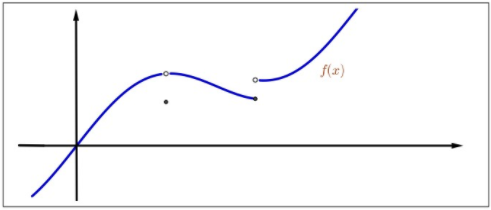
\includegraphics[width=0.7\textwidth]{figs/lowersemi.png} %插入图片,[]中设置图片大小,{}中是图片文件名
\caption{Lower semi-continuity} %最终文档中希望显示的图片标题
\label{Fig.main2} %用于文内引用的标签
\end{figure}
\begin{figure}[H] %H为当前位置,!htb为忽略美学标准,htbp为浮动图形
\centering %图片居中
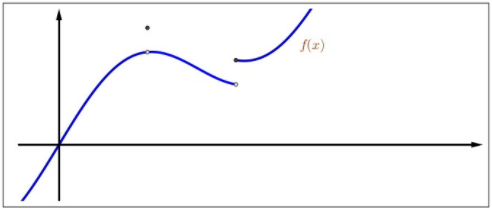
\includegraphics[width=0.7\textwidth]{figs/highersemi.png} %插入图片,[]中设置图片大小,{}中是图片文件名
\caption{Higher semi-continuity} %最终文档中希望显示的图片标题
\label{Fig.main2} %用于文内引用的标签
\end{figure}
\bibliography{robust}
\bibliographystyle{apalike}
\end{document}

